%%%%%%%%%%%%%%%%%%%%%%%%%%%%%%
% 週報フォーマット
% 神経情報システム研究室
%%%%%%%%%%%%%%%%%%%%%%%%%%%%%%
\documentclass[dvipdfmx, A4j, twocolumn, 10.5pt]{jsarticle}
% \usepackage[doublespacing]{setspace} % ダブルスペースにしたいときはコメントを外す
\usepackage[margin=20truemm]{geometry} % 上下左右の余白は2cm
\usepackage{graphicx} % 図を挿入
\setlength{\columnsep}{2zw} % 列の間の空白



\usepackage{amsmath} % 数式?
% \usepackage{caption} % キャプションの追加
% \usepackage{biblatex} % 参考文献を扱うパッケージ
\usepackage{comment} % コメントを挿入する


% \addbibresource{references.bib} % リソースを取得


\begin{document}
%\thispagestyle{empty} % ページ番号はいらない

%%% タイトルなど
\twocolumn[%

\centering % 中央寄せ
{\fontsize{18pt}{18pt}\selectfont 週報}\\ % 和文題目
{\fontsize{12pt}{12pt}\selectfont 2024/06/24} \\
{\fontsize{12pt}{12pt}\selectfont tat}
\vskip\baselineskip % 一行空け
] 

%%% 本文
\section{先週やったこと}
\begin{itemize}
 \item 『神経回路シミュレーション』山崎匡 読み進め
 \item Hodgkin-Huxley方程式にガウスノイズを入れた研究のサーチ

\end{itemize}
\section{『神経回路シミュレーション』要約}


\section*{第3章 神経回路シミュレーション入門}

ニューロンとシナプスの微分方程式による記述と,常微分方程式の数値解法を説明したところで,実際にシミュレーションのプログラムを作成していく.


\subsection*{3.1 ホジキン・ハクスレーモデルのシミュレーション}


\subsection*{3.2 積分発火型モデルのシミュレーション}
\subsubsection*{3.2.1 積分発火型モデル}

HHモデルは,実際のニューロンのメカニズムに忠実な分,
\begin{itemize}
 \item V,m,h,nと,変数を4つも用いる
 \item スパイクが素早いダイナミクスを取る為,刻み幅を小さく取る必要がある
\end{itemize}

といった問題がある.脳の情報処理において重要なのはスパイクの発火頻度やタイミングにあり,スパイクの波形自体には情報はないと考えられている.そのような前提に立った上で,1変数のみを用い,刻み幅を比較的粗くとれるシンプルなニューロンモデルとして,積分発火型(Leaky Integrate-and-Fire, LIF)モデルがある.

LIF モデルは次の式で記述される.

$$
\begin{gathered}
\tau \frac{d v}{d t}=-\left(v(t)-V_{\text {rest }}\right)+R I_{\text {ext }}(t) \\
v(t)>\theta \Rightarrow S(t)=1, v(t) \leftarrow V_{\text {reset }} \\
v(0)=V_{\text {init }}
\end{gathered}
$$

 \begin{itemize}
    \item $v(t)[\mathrm{mV}]$: 時刻 $t$ における膜電位
    \item $\tau[\mathrm{ms}]$: 時定数\footnote{ある値に変化するまでにかかる時間}
    \item $V_{\text {rest }}[\mathrm{mV}]$: 静止電位
    \item $R$ $[\mathrm{M} \Omega]$: 膜の抵抗
    \item $I_{\mathrm{ext}}(t)[\mathrm{nA}]$: 外部電流
    \item $\theta[\mathrm{mV}]$: スパイクを発射する閾値
    \item $V_{\text {reset }}[\mathrm{mV}]$: リセット電位
    \item $V_{\text {init }}[\mathrm{mV}]$: 膜電位の初期値
 \end{itemize}



1つ目の式が,膜電位のダイナミクスを表現する.ここで,HHモデルの数式を再度確認する.

$$
\begin{aligned}
C \frac{d V}{d t}= & -\bar{g}_{\text {leak }}\left(V(t)-E_{\text {leak }}\right)-g_{\mathrm{Na}}(V, t)\left(V(t)-E_{\mathrm{Na}}\right) \\
&  -g_{\mathrm{K}}(V, t)\left(V(t)-E_{\mathrm{K}}\right) +I_{\text {ext }}(t)
\end{aligned}
$$

HHモデルでは,イオンチャネルのコンダクタンス$g_{\mathrm{Na}}(V, t), g_{\mathrm{K}}(V, t)$ を考慮していたが,LIFモデルにはこれらを考慮しない.

$$
\begin{aligned}
C \frac{d V}{d t}= & -\bar{g}_{\text {leak }}\left(V(t)-E_{\text {leak }}\right) +I_{\text {ext }}(t)
\end{aligned}
$$

この両辺に $1 / \bar{g}_{\text {leak }}$ をかけると, $R=1 / \bar{g}_{\text {leak }}$ に注意すればLIFモデルの式が得られる。



ここで,左辺のキャパシタンス$C$について,

$$
\begin{aligned}
& C[F]=\frac{Q[C]}{V[V]} \\
& g[S]=\frac{1}{R[\Omega]}\left(=\frac{I[A]}{V[V]}\right\) \\
& C[F] \times \frac{1}{g[S]}=\frac{Q[C]}{I[A]}=\tau 
\end{aligned}
$$
 \footnote{この数式に基づけば,時定数$\tau$は,電荷$Q$が流れるのに要する時間と解釈できる}

以上のようにして時定数$\tau[\mathrm{ms}]$が得られる.このような,コンダクタンスを陽に記述しないモデルをカレントベースモデルといい\footnote{キャパシタンスやコンダクタンスを記述するLIFモデルも存在するため,必ずしも,LIFモデル=カレントベースというわけではない.},HHモデルのような陽に記述するモデルをコンダクタンスベースモデルという.以上の表現により,LIFモデルは膜電位のみを変数とするモデルであることがわかる.

またスパイク生成も,膜電位の閾値とリセット電位で表現するため,実際のスパイクのダイナミクスは考慮しておらず,したがって,刻み幅もHHモデルの$10[\mu \mathrm{s}]$に対して,$1[\mathrm{ms}]$と,100倍の幅で取ることができる.


膜電位は $V_{\text {rest }}$ を平衡点とし,外部入力 $R I_{\text {ext }}(t)$ を加えた $V_{\text {rest }}+R I_{\text {ext }}(t)$ に時定数 $\tau$ で漸近する挙動を示す.次の式は,スパイク発射の条件である.膜電位が閾値を超えると,その時刻でスパイクを発射したものとし $(S(t)=1)$, かつ膜電位をリセットする.最後の式は膜電位の初期値を与える.

\vspace{\baselineskip}

\subsubsection*{3.2.2 LIFモデルのシミュレーション}
実際にこれらを実装した下のコードを用いて,LIFモデルの1ニューロンのシミュレーションを行うと,次のようなスパイク発射の様子が確認できる.

\begin{figure}[h]
    \centering
    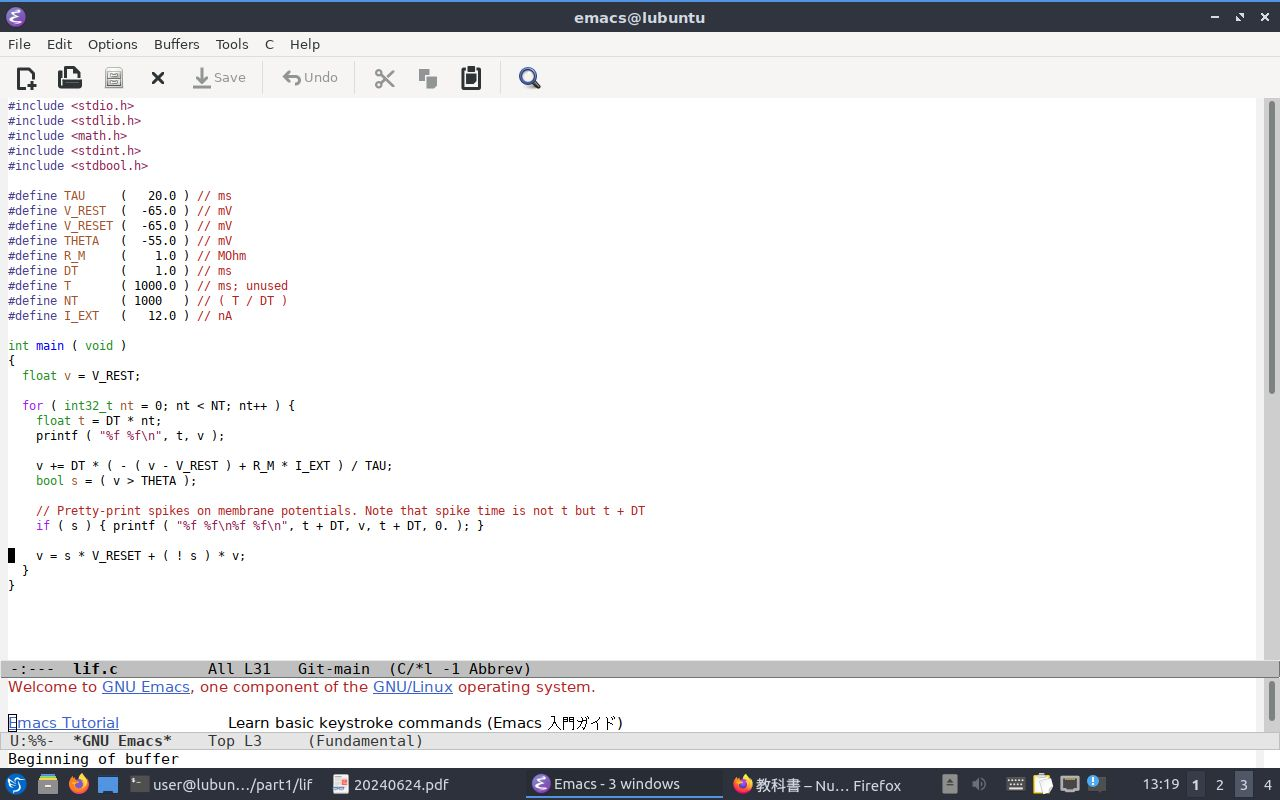
\includegraphics[width=0.5\textwidth]{images/lif_c.jpg}
    \caption{lif.c}
\end{figure}

\begin{figure}[h]
    \centering
    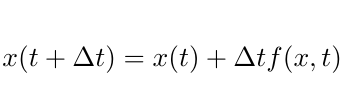
\includegraphics[width=0.5\textwidth]{images/euler.png}
    \caption{オイラー法による$\Delta t$秒後の値の更新}
\end{figure}

\begin{figure}[h]
    \centering
    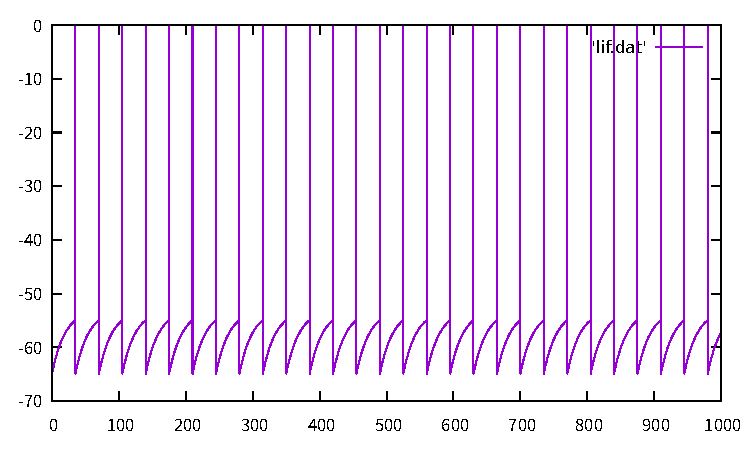
\includegraphics[width=0.5\textwidth]{images/lif.pdf}
    \caption{1000ms間の計算結果}
\end{figure}

\begin{figure}[h]
    \centering
    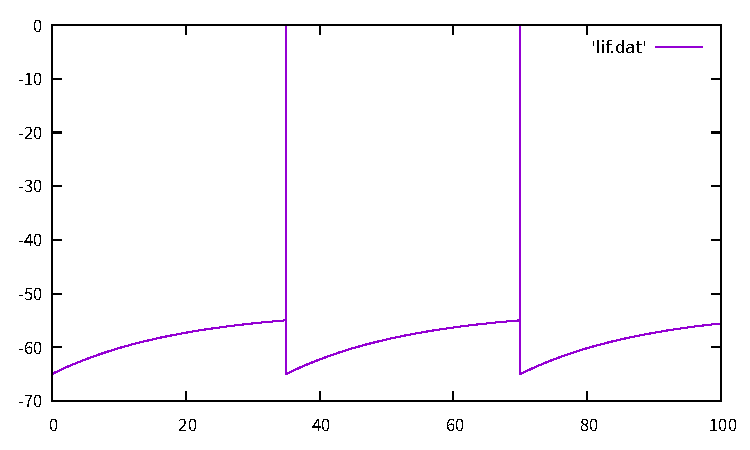
\includegraphics[width=0.5\textwidth]{images/lif_100ms.pdf}
    \caption{100ms間の計算結果}
\end{figure}

HHモデルを用いたシミュレーションにおいては,4次ルンゲクッタ法を用いていたが,今回のLIFモデルを用いたシミュレーションでは比較的誤差の大きいオイラー法を使用し,また,刻み幅も$0.01[\mathrm{ms}]$($10\mathrm{\mu s}]$)から,$1[\mathrm{ms}]$と100倍になっている.結果,ループの回転数は1/100,ループ1回あたりの浮動小数点演算数も1/100になり,単純計算で総演算数は1/10000以下まで減少している.波形を確認すると,スパイクのダイナミクスは表現されていないことが見て取れる.

\subsubsection*{3.2.4 不応期の導入}
スパイク後,膜電位の値がもとの静止電位の値よりも低くなり,一定時間スパイクを発射しなくなる不応期はカリウムイオンチャネルのコンダクタンス上昇によりカリウムイオンが細胞外へ流出することにより発生していたが,今回のLIFモデルにおいてはカレントベースのモデルであるためコンダクタンスの変化は反映されておらず,不応期は見られない.人工的に導入する方法として,膜電位の値を一定時間強制的に$V_{\text {rest }}[\mathrm{mV}]$に固定する方法がある.

\begin{figure}[h]
    \centering
    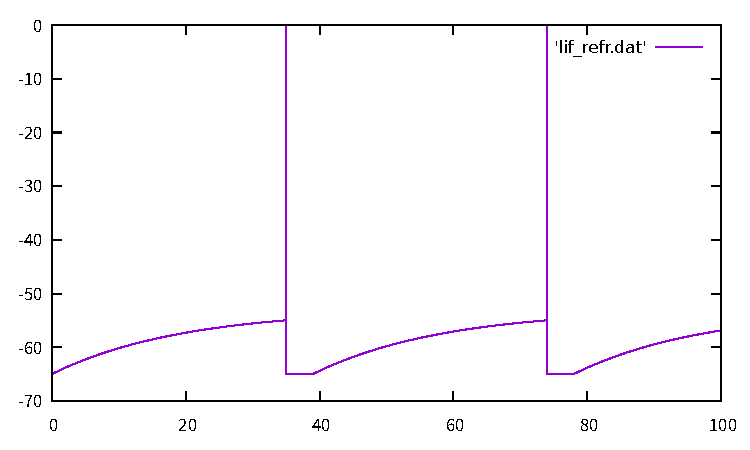
\includegraphics[width=0.5\textwidth]{images/lif_refr_100ms.pdf}
    \caption{100ms間の計算結果(不応期の導入)}
\end{figure}

\begin{figure}[h]
    \centering
    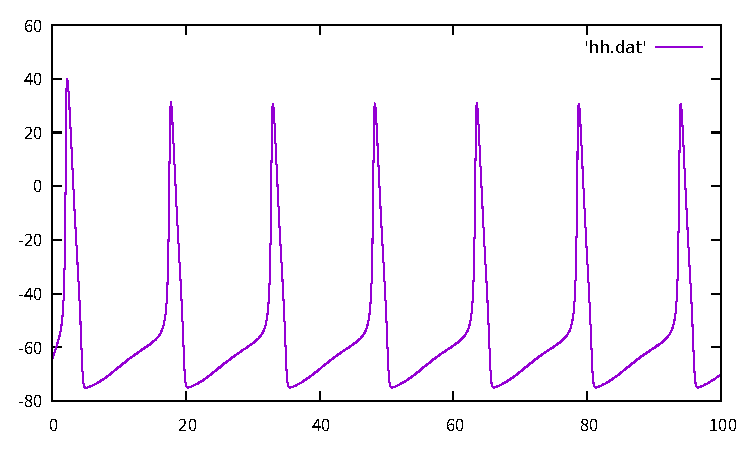
\includegraphics[width=0.5\textwidth]{images/0301_hh_100.pdf}
    \caption{(参考)100msの計算結果(HHモデルの場合)発火頻度の相違は,入力電流の相違によるもの.}
\end{figure}

これはあくまでの人工的な実装であり,実際のダイナミクスではないことに注意する(実際,今回の方法では,不応期において元の静止電位-65mVよりも小さい値を取る現象については表現されていない).参考までに前回示したHHモデルで得られた波形も示す\footnote{LIFとHHで発火頻度が異なるのは単に入力電流の違いによるものである.}.

\vspace{\baselineskip}
\vspace{\baselineskip}

\section{Paper: 確率論的HHにおけるスパイク列}

(略)

\vspace{\baselineskip}
\vspace{\baselineskip}

\section*{Other}
*よくわかっていない点 \\

・反転電位「E」\\

→どうしてHHモデルの反転電位「E」の箇所が,LIFモデルでは静止電位「Vrest」に置き換わるのかがわからない.\\

*この時期から論文を読み進めるべきか \\

・英語がわからない \\

・(異言語以前に)知識量の問題で内容が分かってない \\

・読解力がない \\

の,三重苦で文脈とかがいちいち汲み取れず,全体として何をいってるのかわからない.例えば,「外部電流にガウスノイズを入力する」という文章があっても,実際にコードを動かしてシミュレーションをした経験が乏しいため,何をやってるのかが漠然としていて,その浮遊感のまま読み勧めても結局何をやってるのかあまり理解できてない.正直前期のあいだは(院試等もあるので)『神経回路シミュレーション』に一通り取り組んでから論文とかに着手したいが,中間発表や芝浦の一般入試の面談に先立って研究テーマに直結する論文とかは一定度把握しておくべきか.






\section{今週やること}
\begin{itemize}
 \item ??
 \item ??
\end{itemize}




\begin{thebibliography}{99}
% \bibitem{lite1} 和田勝 ``筋肉による筋収縮の司令'' 生命科学C, 2001, https://www.tmd.ac.jp/artsci/biol/textlife/neuron.html.
% \bibitem{lite2} R. Hosaka, T. Kimura, and T. Matsuura, ``title,'' journal name, pp.10-20, 2021.
\bibitem{lite2} Henry C. Tuckwell, ``Spike trains in a stochastic Hodgkin–Huxley system(確率論的HHにおけるスパイク列)'' Biosystems, 2005, https://www.sciencedirect.com/science/article/abs/pii/S0303264704001716?via%3Dihub
\end{thebibliography}
\end{document}
